\documentclass{bredelebeamer}

%%%%%%%%%%%%%%%%%%%%%%%%%%%%%%%%%%%%%%%%%%%%%%%%

\title[Programación en MatLAB]{Introducción a la programación con MatLAB}
\subtitle{Módulo 07 - Entrada y salida definida por el usuario}

\author{Autor1 - Autor2 - Autor3\inst{1}}
\institute[UTN.BA]
{
  \inst{1}%
  Universidad Tecnológica Nacional\\
  Facultad Regional Buenos Aires
  }

\date{dia mes 2018}

\subject{Taller de programación}

\logo{

\includegraphics[scale=0.15]{images/logo.png}
}

%%%%%%%%%%%%%%%%%%%%%%%%%%%%%%%%%%%%%%%%%%%%%%%%%%%%%%%%%%%%%%%%%%%%%
\begin{document}

\begin{frame}
  \titlepage 
\end{frame}


%%%%%%%%%%%%%%%%%%%%%%%%%%%%%%%%%%%%%%%%%%%%%%%%%%%%%%%%%%%%%%%%%%%%%

% Entrada y salida controlada por el usuario

%%%%%%%%%%%%%%%%%%%%%%%%%%%%%%%%%%%%%%%%%%%%%%%%%%%%%%%%%%%%%%%%%%%%%

\section{Entrada y salida controlada por el usuario}

\begin{frame}{Entrada y salida controlada por el usuario}
Primera clase:
\begin{itemize}
\item Matlab como memoria de trabajo auxiliar (ventana de comandos)
\item Desarrollo de programas simples
\begin{itemize}
\item Script
\item Funciones internas de matlab
\end{itemize}
\end{itemize}
El objetivo de la clase es la realización de programas más complicados suponiendo que el \textbf{programador y el usuario} son personas diferentes
\end{frame}

\begin{frame}{Entrada definida por el usuario}
\begin{exampleblock}{Comando}
Ver comando: \textbf{input()}
\end{exampleblock}
La función \textbf{input} despliega una cadena de texto en la ventana de comando y luego espera que el usuario proporcione la entrada solicitada.
\end{frame}

\begin{frame}{Entrada definida por el usuario}
Ej. Ejecutar las siguientes líneas. Obtener conclusiones.
\boiteviolette{
\begin{center}
z = input('Ingresar un valor');
\end{center}
}
\begin{columns}
\begin{column}{0.5\textwidth}
\begin{center}
Command windows
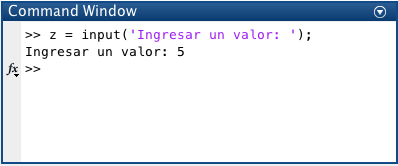
\includegraphics[scale=0.3]{images/pantalla1.png}
\end{center}
\end{column}
\begin{column}{0.3\textwidth}
\begin{center}
Workspace
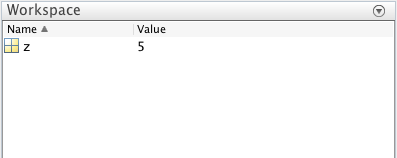
\includegraphics[scale=0.3]{images/pantalla2.png}
\end{center}
\end{column}
\end{columns}
\begin{block}{Tener en cuenta}
Puede ingresarse matrices, cadena de caracteres, entre otros.
\end{block}
\end{frame}

\begin{frame}{Ejercicio práctico 1}
\begin{enumerate}
\item Cree un archivo .m para calcular el área de un triángulo. Permita al usuario ingresar los valores para la base y la altura.
\item Cree un archivo .m para encontrar el volumen de un cilíndro circular recto.
\item Cree un vector desde 1 hasta n, y permita al usuario ingresar el valor de n.
\item Cree un vector que comience en a, termine en b y tenga un espacio de c. Permita al usuario ingresar todos estos parámetros.
\end{enumerate}
\end{frame}

\begin{frame}{Opciones de salida}
\begin{center}
Primera forma de desplegar contenidos de una matriz
\end{center}
Ej. Ejecutar las siguientes líneas. Obtener conclusiones.
\boiteviolette{
\begin{center}
x = 1:5;\\
x
\end{center}
}
\end{frame}

\begin{frame}{Opciones de salida}
\begin{center}
Segunda forma de desplegar contenidos de una matriz
\end{center}
\begin{exampleblock}{Comando}
Ver comando: \textbf{disp(x)}
\end{exampleblock}
La función \textbf{disp} despliega los contenidos de una matriz sin imprimir el nombre de matriz.\\
Ej. Ejecutar las siguientes líneas. Obtener conclusiones.
\boiteviolette{
x = 1:5;\\
disp(x);
}
\begin{block}{Tener en cuenta}
Puede utilizarse para desplegar una cadena (texto encerrado por comillas simples)
\end{block}
\end{frame}


\begin{frame}{Opciones de salida}
Ej. Ejecutar las siguientes líneas. Obtener conclusiones.
\boiteviolette{
x = 1:5;\\
disp('Los valores de x son: ');\\
disp(x);
}
\begin{block}{Tener en cuenta}
Las dos funciones disp se despliegan en líneas separadas.
\end{block}
\end{frame}

\begin{frame}{Opciones de salida}
Utilizando la función \textbf{num2str(x)} y concatenando dos cadenas \textbf{[cadena1 cadena2]} se obtiene una salida en una única línea.\\
Ej. Ejecutar las siguientes líneas. Obtener conclusiones.
\boiteviolette{
x = 1:5;\\
disp(['Los valores de x son: ' num2str(x)]);
}
\begin{exampleblock}{Comando}
Ver comando: \textbf{num2str(x)}
\end{exampleblock}
La función \textbf{num2str} cambia un arreglo de números en un arreglo de caracteres.
\end{frame}

\begin{frame}{Salida formateada}
La función \textbf{fprintf} además de desplegar los valores (\textit{ver función dis} permite especificar el formato y saltos de línea.
\begin{exampleblock}{Comando}
Ver comando: \textbf{fprintf(x)}
\end{exampleblock}
Ej. Ejecutar las siguientes líneas. Obtener conclusiones.
\boiteviolette{
cantidad = 5;\\
fprintf('Hay \textbf{\%f} personas en mi casa',cantidad);
}
\end{frame}

\begin{frame}{Marcadores de posición}
\begin{table}[]
\centering
\begin{tabular}{|c|c|}
\hline
Tipo de campo & Resultado                      \\ \hline
\%f           & Notación punto fijo o decimal  \\ \hline
\%e           & Notación exponencial           \\ \hline
\%g           & La que sea más corta \%f ó \%e \\ \hline
\%c           & Información carácter           \\ \hline
\%s           & Cadena de caracteres           \\ \hline
\end{tabular}
\end{table}
\end{frame}

\begin{frame}{Salida formateada}
Ej. Ejecutar las siguientes líneas. Obtener conclusiones.
\boiteviolette{
cantidad = 5;\\
fprintf('Hay \textbf{\%f} personas en mi casa',cantidad);\\
cantidad = 7;\\
fprintf('Hay \textbf{\%f} personas en tu casa',cantidad);
}
\end{frame}

\begin{frame}{Salida formateada}
\begin{block}{Tener en cuenta}
Para indicar nueva línea utilizar el comando de formato: \textbf{\textbackslash n}
\end{block}
Ej. Ejecutar las siguientes líneas. Obtener conclusiones.
\boiteviolette{
cantidad = 5;\\
fprintf('Hay \textbf{\%f} personas en mi casa \textbf{\textbackslash n}',cantidad);\\
cantidad = 7;\\
fprintf('Hay \textbf{\%f} personas en tu casa \textbf{\textbackslash n}',cantidad);
}
\end{frame}

\begin{frame}{Comandos de formato}
\begin{table}[]
\centering
\begin{tabular}{|c|c|}
\hline
Comando de formato & Acción resultante     \\ \hline
\textbackslash{}n  & Salto de línea        \\ \hline
\textbackslash{}r  & Regreso de carro      \\ \hline
\textbackslash{}t  & Tabulador             \\ \hline
\textbackslash{}b  & Retroceder un espacio \\ \hline
\end{tabular}
\end{table}
\end{frame}

\begin{frame}{Width field y precision field}
\begin{itemize}
\item Width field: Controla el número mínimo de caracteres a imprimir con el comando format.
\item Precision field está precedido por un punto (.) y especifica el número de lugares decimales después del punto decimal.
\end{itemize}
Ej. Ejecutar las siguientes líneas. Obtener conclusiones.
\boiteviolette{
voltaje = 3.5;\\
fprintf('El voltage es \textbf{\%8.2f}\textbackslash n',voltaje);
}

\begin{alertblock}{Importante}
Si quiere incluir signo de porcentaje en un enunciado fprintf, se debe ingresar \%\% dos veces de lo contrario se interpretara \% como marcador de posición para datos.
\end{alertblock}
\end{frame}

%%%%%%%%%%%%%%%%%%%%%%%%%%%%%%%%%%%%%%%%%%%%%%%%%%%%%%%%%%%%%%%%%%%%%

% Sección de consultas

%%%%%%%%%%%%%%%%%%%%%%%%%%%%%%%%%%%%%%%%%%%%%%%%%%%%%%%%%%%%%%%%%%%%%

\section{Consultas}
\begin{frame}{Consultas}
\begin{center}

\includegraphics[scale=0.3]{images/consultas.png}
\end{center}
\end{frame}


%%%%%%%%%%%%%%%%%%%%%%%%%%%%%%%%%%%%%%%%%%%%%%%%%%%%%%%%%%%%%%%%%%%%%

% Sección de bibliografía

%%%%%%%%%%%%%%%%%%%%%%%%%%%%%%%%%%%%%%%%%%%%%%%%%%%%%%%%%%%%%%%%%%%%%

\section{Bibliografia}

\begin{frame}{Bibliografía}
\begin{columns}
\begin{column}{0.5\textwidth}
\begin{center}

\includegraphics[scale=0.4]{images/biblio1.png}
\end{center}
\end{column}
\begin{column}{0.5\textwidth}
\begin{center}
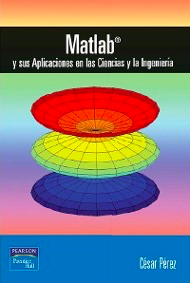
\includegraphics[scale=0.5]{images/biblio2.png}
\end{center}
\end{column}
\end{columns}
\end{frame}

\end{document}
